\documentclass[14pt, oneside]{altsu-report}

\worktype{ОТЧЁТ ПО ТЕХНОЛОГИЧЕСКОЙ (ПРОЕКТНО-ТЕХНОЛОГИЧЕСКОЙ)
ПРАКТИКЕ НА ТЕМУ:}
\title{Разработка игры «Арканоид» на python}
\author{М.\,С.~Дягилев}
\groupnumber{5.205-2}
\GradebookNumber{1337}
\supervisor{И.\,А.~Шмаков}
\supervisordegree{ст.преп.}
\ministry{Министерство науки и высшего образования}
\country{Российской Федерации}
\fulluniversityname{ФГБОУ ВО Алтайский государственный университет}
\institute{Институт цифровых технологий, электроники и физики}
\department{Кафедра вычислительной техники и электроники}
\departmentchief{В.\,В.~Пашнев}
\departmentchiefdegree{к.ф.-м.н., доцент}
\shortdepartment{ВТиЭ}
\abstractRU{ 
Объект исследования: Языки программирования

Предмет исследования: Язык программирования Python и библиотеки PySide6. Разработка игры с применением объектно-ориентированного программирования, графического интерфейса пользователя (GUI) и игровой логики.

Цель работы: Разработка игры на Python c использованием библиотеки PySide6. 
}
\abstractEN{Большой текст на английском!}
\keysRU{Python, PySide6, программирование, GUI}
\keysEN{computer simulation, distributed version control}

\date{\the\year}

% Подключение файлов с библиотекой.
\addbibresource{graduate-students.bib}

% Пакет для отладки отступов.
%\usepackage{showframe}

\begin{document}
\maketitle

\setcounter{page}{2}
\makeabstract
\tableofcontents

\chapter*{Введение}
\phantomsection\addcontentsline{toc}{chapter}{ВВЕДЕНИЕ}

\textbf{Актуальность} 
\begin{enumerate}

\item Изучение языка программирования Python и библиотеки PySide6:

Изучение Python, а также библиотеки PySide6 для разработки GUI, способствует развитию навыков программирования, логического мышления и алгоритмизации. 

\item Создание функционального приложения:

Разработка приложений с использованием PySide6 позволяет создавать функциональные приложения с графическим интерфейсом пользователя.

\item Овладение навыками создания GUI:

Использование PySide6 обеспечивает возможность разработки красивых и интуитивно понятных пользовательских интерфейсов. 

\item Развитие программной индустрии:

В современном мире разработка программного обеспечения с GUI становится все более востребованной.
\end{enumerate}

\textbf{Цель}

Целю игры является создание игры "Арканоид" на языке Python c использованием библиотеки PySide6.

\textbf{Задачи:}
\begin{enumerate}
\item Реализовать игровые элементы:
\begin{itemize}
    \item Платформа.
    \item Мяч.
    \item Кирпичики.
\end{itemize}
\item Игровой процесс
\begin{itemize}
    \item Обрабатывать столкновение мяча с платформой и кирпичиками.
    \item Изменять направление мяча после столкновения.
    \item Завершать игры после достижении мячом нижней границы.
    \item Реализовать управление платформой с помощью мыши.
\end{itemize}
\item Меню
\begin{itemize}
    \item Кнопка "Играть"
    \item Кнопка "Help"
\end{itemize}
\end{enumerate}

% Подключение первой главы (теория):
\chapter{\label{ch:ch01}ГЛАВА 1} % Нужно сделать главу в содержании заглавными буквами

\section{\label{sec:ch01/sec01} Арканоид}

\subsection{\label{subsec:ch01/sec01/sub01}Об игре}
***что такое "Арканоид" и какие правила игры.***
Пример <<ковычек>> и тире ---.

Пример нумерованного списка:
\begin{enumerate}
\item Первый элемент.
\item Второй элемент.
\end{enumerate}

\subsection{\label{subsec:ch01/sec01/sub02}Цель игры и основные механики}
***Объяснить цель игры и основные механики.***
Пример маркерованного списка:
\begin{itemize}
\item первый элемент;
\item второй элемент.
\end{itemize}

\section{\label{sec:ch01/sec02}Раздел 2: Python}
    
\subsection{\label{subsec:ch01/sec02/sub01}Теория Python}
***Рассказать о языке питон, почему был выбран именно он и т.д***
Пример вложенного нумерованного списка:
\begin{enumerate}
\item Первый элемент:
\begin{enumerate}
\item Первый элемент первого элемента;
\item Второй элемент первого элемента;
\end{enumerate}
\item Второй элемент:
\begin{enumerate}
\item Первый элемент второго элемента;
\item Второй элемент второго элемента.
\end{enumerate}
\end{enumerate}

\subsection{\label{subsec:ch01/sec02/sub02}PySide}
*** описать, что такое PySide6 и для чего она используется.***
***Упомянуть основные возможности и преимущества использования PySide6.***
Пример вложенного маркерованного списка:
\begin{itemize}
\item первый элемент:
\begin{itemize}
\item первый элемент первого элемента;
\item второй элемент первого элемента;
\end{itemize}
\item Второй элемент:
\begin{itemize}
\item первый элемент второго элемента;
\item второй элемент второго элемента.
\end{itemize}
\end{itemize}


% Подключение второй главы (практическая часть):
\chapter{\label{ch:ch02}РЕАЛИЗАЦИЯ ИГРЫ АРКАНОИД}

\section{\label{sec:ch02/sec01}Техническое задание}
Основное окно меню содержит кнопки "Play", "Help" и "Exit". Код в кнопке "Help" содержит создание окна с информацией об игре "Арканоид". Когда окно игры "Arkanoid" открывается после нажатия на кнопку "Play", пользователь увидит интерактивную сцену, на которой развернут классический игровой процесс этой игры. Вот краткое описание окна игры:
\begin{itemize}
    \item \textbf{Игровая сцена:}
    
        Верхняя часть экрана занята рядами кирпичей разных цветов и типов, которые игрок должен разрушить мячом. В нижней части экрана расположена подвижная платформа, которую управляет пользователь с помощью мыши. Внизу экрана показывается платформа и мяч, который начинает движение при клике левой кнопкой мыши.

    \item \textbf{Интерфейс:}
    
        Справа от игровой сцены расположены индикаторы жизней игрока в виде кругов. Вверху экрана расположена надпись "Score", отображающая текущий счет игрока в реальном времени. 
\end{itemize}
\section{\label{sec:ch02/sec02}Основные модули и функции}

\subsection{\label{subsec:ch02/sec02/sub01}Инициализация модулей}
\begin{itemize}
    \item \textbf{PySide6.QtWidgets:}
    Этот модуль предоставляет классы и функции для создания интерактивных пользовательских интерфейсов (GUI) в Qt6. В коде используются классы QApplication, QMainWindow, QWidget, QHBoxLayout, QVBoxLayout, QPushButton, QLabel, QGraphicsScene, QGraphicsView, QGraphicsRectItem, и QGraphicsEllipseItem для создания графического интерфейса игры и ее меню.

    \item \textbf{PySide6.QtCore:}
    Модуль QtCore содержит ядро Qt, включая базовые классы и функциональность. В коде используются классы Qt, QTimer для работы с событиями и таймером.

    \item \textbf{PySide6.QtGui:} 
    Этот модуль содержит классы для работы с графическими элементами в Qt6. В коде используется класс QFont для установки шрифтов, QPen для рисования контуров, QColor для работы с цветами.

    \item \textbf{random:} ~\cite{wikigeeksforgeeks}
    Встроенный модуль Python для генерации случайных чисел и выборки случайных элементов. В коде используется для различных случайных операций, таких как распределение бонусов и создание случайного размещения блоков.
    
\end{itemize}



\subsection{\label{subsec:ch02/sec02/sub02}Описание основных классов}
Вся структура класса «\textbf{ArkanoidMainMenu}» обеспечивает создание и управление элементами интерфейса главного меню игры Arkanoid, обеспечивая пользователя информацией о доступных опциях (игра, помощь, выход). Это позволяет пользователям удобно навигироваться и взаимодействовать с приложением до начала самой игры. 

Класс «\textbf{ArkanoidGame}» представляет игровой экран Arkanoid, использует QGraphicsView и QGraphicsScene для отрисовки игровых объектов.

Основные атрибуты и методы:
\begin{itemize}
    \item platform: Платформа, которую управляет игрок.
    \item ball: Мяч, который отскакивает от блоков и платформы.
    \item bricks: Список кирпичей, которые нужно разрушить.
    \item bonuses: Список бонусов, которые могут выпасть из блоков.
    \item generate\_bricks(): Генерирует кирпичи на игровом поле. Создает QGraphicsRectItem для каждого кирпича случайным образом, устанавливает их позицию и цвет, добавляет на сцену.
    \item update(): Обновляет состояние игры при каждом тике таймера. Обрабатывает движение мяча, столкновения с платформой и кирпичами, проверяет условия победы или поражения, обновляет счетчик жизней и очков.
    \item mouseReleaseEvent(): Обрабатывает событие клика мыши для начала игры. При первом клике начинает движение мяча и запускает игру.
    \item apply\_bonus(): Применяет бонус, выпавший из блока. Изменяет свойства игровых элементов в зависимости от типа бонуса (увеличение платформы, изменение цвета мяча).
    \item mouseMoveEvent(): Обрабатывает движение мыши для управления платформой. Перемещает платформу в соответствии с положением мыши, если игра уже началась.
    \item check\_lives(): Проверяет количество жизней игрока. Удаляет индикаторы жизней и отображает главное меню.
    \item check\_restart\_conditions(): Проверяет условия для перезапуска игры. Возвращает мяч и кирпичи в начальное положение, генерирует новую структуру кирпичей.
\end{itemize}

Класс «\textbf{Bonus}»  представляет бонус, который может выпасть из блоков при разрушении. Тип бонуса (увеличение длины платформы, уменьшение длины платформы, усиление мяча).

\subsection{\label{subsec:ch02/sec02/sub03}Генерация блоков}
\textbf{Основные параметры блоков:} 
\begin{itemize}
    \item Размеры блоков:
    \begin{itemize}
        \item Ширина: 75 пикселей
        \item Высота: 20 пикселей
    \end{itemize}

    \item Пространственные параметры:
    \begin{itemize}
        \item Горизонтальный отступ между блоками: 10 пикселя
        \item Вертикальный отступ между блоками: 15 пикселя
    \end{itemize}

    \item Расположение блоков:
    \begin{itemize}
        \item Количество рядов: 5
        \item Количество столбцов: 10
    \end{itemize}
\end{itemize}

\textbf{Процесс генерации:}
    \begin{itemize}
        \item Случайное решение о создании блока:
    
        Для каждой позиции блока генерируется случайное число от 0 до 1. Если случайное число меньше 0.7, создается блок на этой позиции.
    \end{itemize}

\begin{itemize}
    \item Создание и настройка блока:
    
        Создается экземпляр QGraphicsRectItem (блока) с заданными размерами (ширина и высота). Позиция блока вычисляется на основе текущей позиции в сетке, с учетом горизонтального и вертикального отступов. 
        Цвет блока устанавливается в зависимости от случайных вероятностей:
        \begin{itemize}
            \item 0.2 шанс для серого цвета (неразрушаемые блоки)
            \item 0.1 шанс для черного цвета (специальные блоки)
        \end{itemize}
\end{itemize}
\begin{itemize}
    \item Добавление блока на сцену:
    
        После настройки всех параметров блок добавляется на графическую сцену методом self.scene.addItem(brick).
        Экземпляр блока также добавляется в список self.bricks, чтобы можно было в дальнейшем отслеживать и взаимодействовать с ними в игровой логике.
\end{itemize}

\subsection{\label{subsec:ch02/sec02/sub04}Коллизия мяча}
\begin{itemize}
 \item Основные элементы, участвующие в коллизии:
\begin{itemize}
    \item Мяч (self.ball):
    
        Это объект типа QGraphicsRectItem, представляющий мяч на игровой сцене. Его положение и перемещение контролируются в методе update().

    \item Платформа (self.platform):
    
        Также объект типа QGraphicsRectItem, представляющий платформу, которую управляет игрок. Платформа перемещается горизонтально и отскакивает мяч.

    \item Блоки (self.bricks):
    
        Список объектов QGraphicsRectItem, представляющих различные блоки на игровой сцене. Блоки могут быть разрушаемыми и неразрушаемыми (серого и черного цветов).
\end{itemize}
\end{itemize}

\begin{itemize}
\item Обработка коллизий в методе update() ~\cite{book1author1}:
\begin{itemize}
    \item Столкновение с платформой (self.platform):
    
        Когда мяч сталкивается с платформой, проверяется, пересекается ли их ограничивающие прямоугольники (boundingRects).
        Если столкновение обнаружено, происходит изменение направления движения мяча в зависимости от того, с какой стороны платформы мяч ударился: слева, справа, сверху или снизу.

    \item Столкновение с блоками (self.bricks):
    
        Для каждого блока из списка self.bricks проверяется, пересекается ли его ограничивающий прямоугольник с ограничивающим прямоугольником мяча.
        Если столкновение обнаружено и блок разрушаемый (цвет не черный и не серый), блок удаляется со сцены и из списка self.bricks, а игрок получает очки.
        В зависимости от направления столкновения (слева, справа, сверху или снизу), мяч отскакивает в противоположном направлении.
        collision\_occurred отмечаем, что произошло столкновение или нет.
\end{itemize}
\end{itemize}

\subsection{\label{subsec:ch02/sec02/sub05}Бонусы}
\begin{itemize}

    \item Типы бонусов:
    \begin{itemize}
        
        \item Увеличение размера платформы: Этот бонус увеличивает горизонтальный размер платформы, что делает ее более эффективной в отбивании мяча.
        \item Уменьшение размера платформы: Напротив, этот бонус уменьшает горизонтальный размер платформы, что усложняет управление и добавляет сложность в игру.
        \item Усиление мяча: Бонус, который изменяет свойства мяча, делая его более мощным при разрушении блоков (способность разрушать серые блоки).
\end{itemize}        
    \item Визуальное отображение:
    
        Каждый тип бонуса имеет свой уникальный внешний вид, который помогает игроку легко распознать их на игровом поле. Например, зеленый цвет может ассоциироваться с увеличением платформы, красный - с уменьшением, а синий - с усилением мяча.

    \item Сбор бонусов:
    
        Для сбора бонуса платформа игрока должна пересечься с объектом бонуса, пока тот движется вниз по экрану.
        При сборе бонуса применяются соответствующие изменения к игровым параметрам (размер платформы, свойства мяча).
        
\end{itemize}

\section{\label{sec:ch02/sec03}Блок схемы}
Общая блок схема — представлена на рисунке 2.1: 

\begin{figure} [!h]
  \centering
  \graphicspath{ {img/} }
  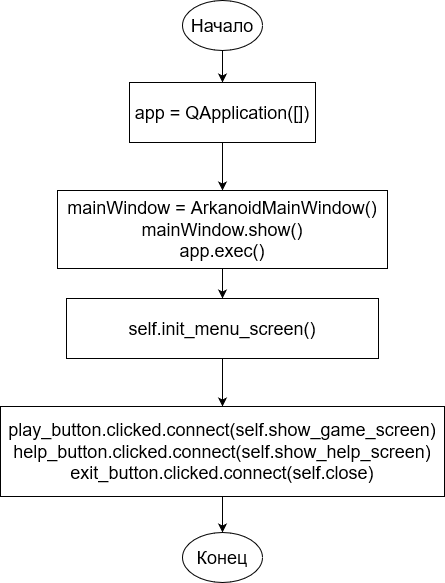
\includegraphics[width = 15cm]{image/11.drawio.png}
  \caption{блок - схема create\_life\_indicators. }
  \label{fig:image}
\end{figure}

Метод create\_life\_indicators создаёт индикаторы жизней для приложения или игры. Блок схема - представлена на рисунке 2.2:

\begin{figure} [!h]
  \centering
  \graphicspath{ {img/} }
  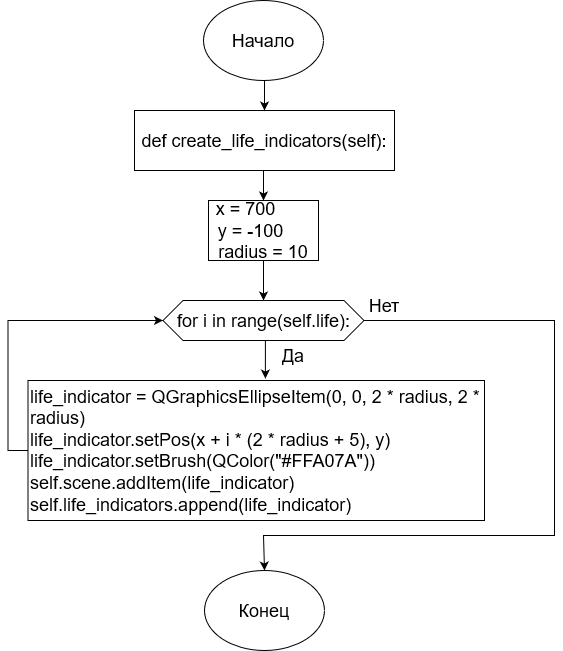
\includegraphics[width = 15cm]{image/22.png}
  \caption{блок - схема create\_life\_indicators. }
  \label{fig:image}
\end{figure}

Этот метод последовательно создаёт круговые индикаторы для каждой жизни игрока, располагая их горизонтально на заданном расстоянии друг от друга.

\section{\label{sec:ch02/sec03}Тестирование}

После открытия схемы должно создаться окно, в котором находятся три кнопки "Play", "Exit", "Help"

\begin{figure}[h!]
    \centering
    \graphicspath{ {img/} }
    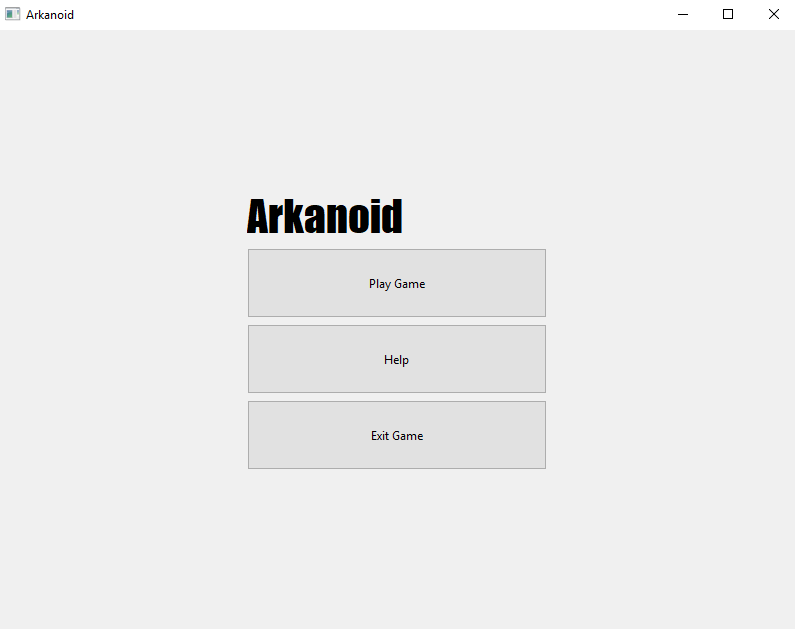
\includegraphics[width = 10cm]{image/1.png}
    \caption{главное меню игры. }
    \label{fig:image}
\end{figure}


После нажатия кнопки "Help" на экране должна появиться информация об игре и кнопка "close".

Проверить кликабельность кнопки "Close" и убедиться, что после клика окно Help закрывается и открывается главное меню.

\begin{figure} [h!]
  \centering
  \graphicspath{ {img/} }
  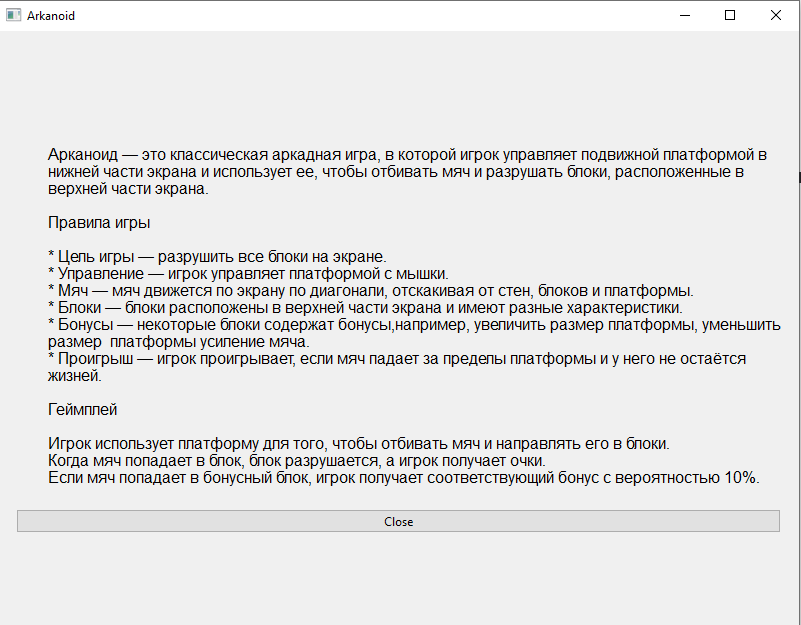
\includegraphics[width=10cm]{image/2.png}
  \caption{Окно "Help". }
  \label{fig:image}
\end{figure}


После нажатия кнопки "Play" На экране должна появиться игра. Проверить, что платформа, мяч и кирпичи отображаются на экране. 

Убедиться, что счет и индикаторы жизней отображаются и начальное значение счета равно 0. 
Проверить, что мяч начинает двигаться после клика мыши.

\begin{figure} [h!]
  \centering
  \graphicspath{ {img/} }
  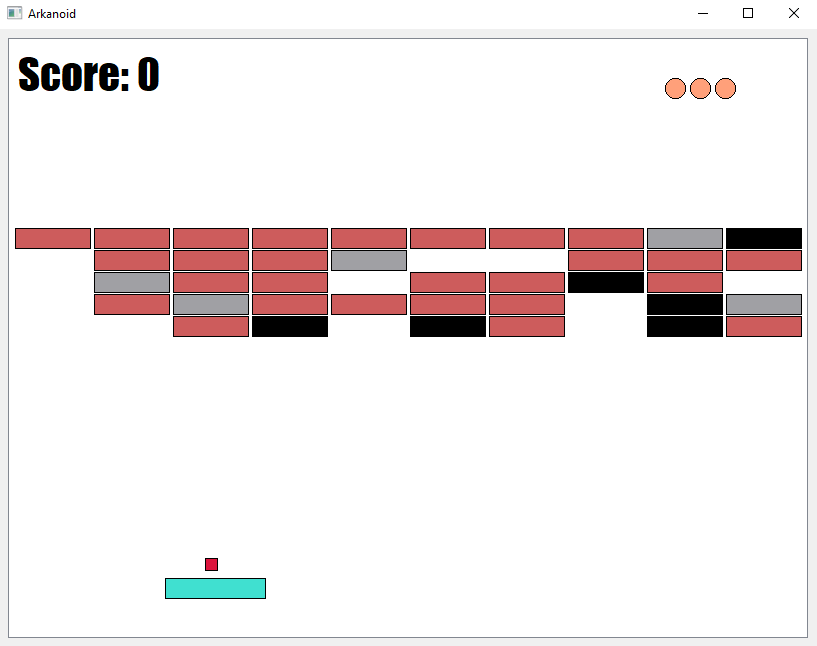
\includegraphics[width=10cm]{image/3.png}
  \caption{окно с игрой. }
  \label{fig:image}
\end{figure}



Проверка индикатора жизней. 

Проверить, что количество отображаемых кругов соответствует начальному количеству жизней. Убедиться, что при потере жизни количество отображаемых индикаторов уменьшается на один. Проверить, что после потери жизни игра возвращает мяч и платформу в начальные позиции, а индикаторы жизней обновляются, и при потере всех жизней игра завершается и возвращается на главное меню.
\clearpage
\begin{figure} [!htp]
  \centering
  \graphicspath{ {img/} }
  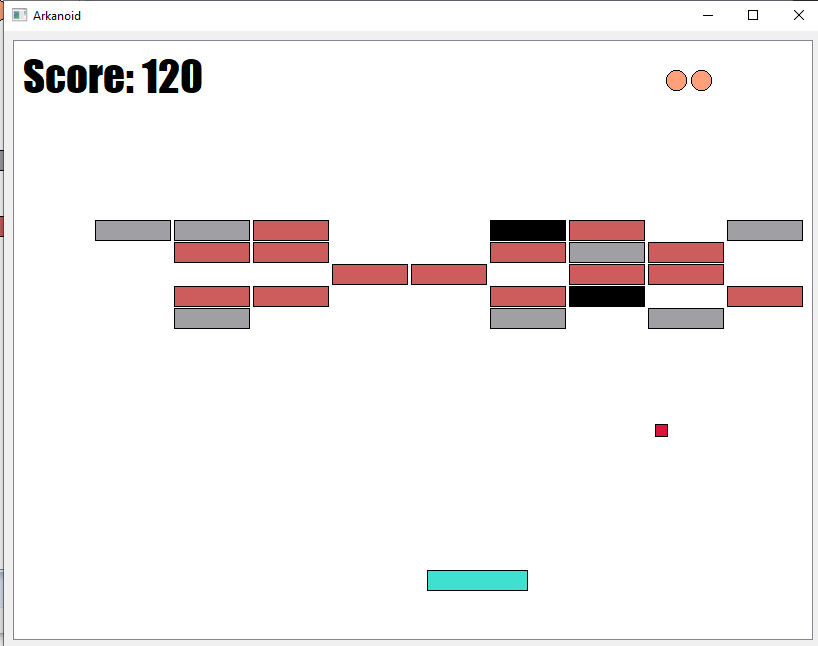
\includegraphics[width=8cm]{image/5.png}
  \caption{окно с игрой (тест индикатора жизней). }
  \label{fig:image}
\end{figure}


Проверка выпадения бонуса. 

Разрушить кирпич с вероятностью выпадения бонуса. Убедиться, что бонус отображается на экране и начинает падать вниз. Проверить, что бонус перемещается по экрану вниз. Убедиться, что бонус исчезает, если он достигает нижней границы экрана или платформы его подбирает.

\begin{figure} [h!]
  \centering
  \graphicspath{ {img/} }
  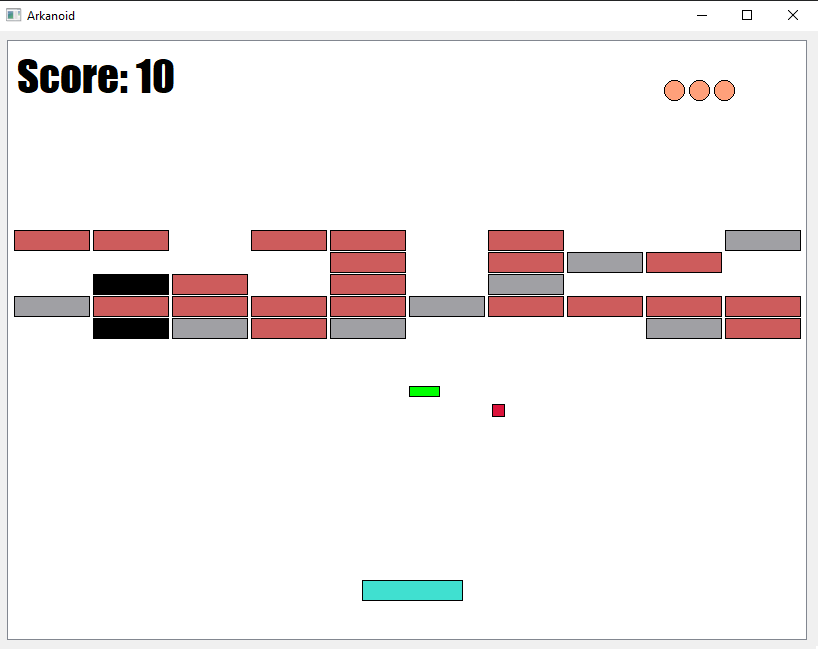
\includegraphics[width=10cm]{image/6.png}
  \caption{окно с игрой (тест выпадения бонуса). }
  \label{fig:image}
\end{figure}

Проверка подбора бонуса. 

Убедиться, что платформа подбирает бонус и его эффект немедленно применяется.
Проверить, что размер платформы изменяется в зависимости от типа бонуса.

\begin{figure} [h!]
  \centering
  \graphicspath{ {img/} }
  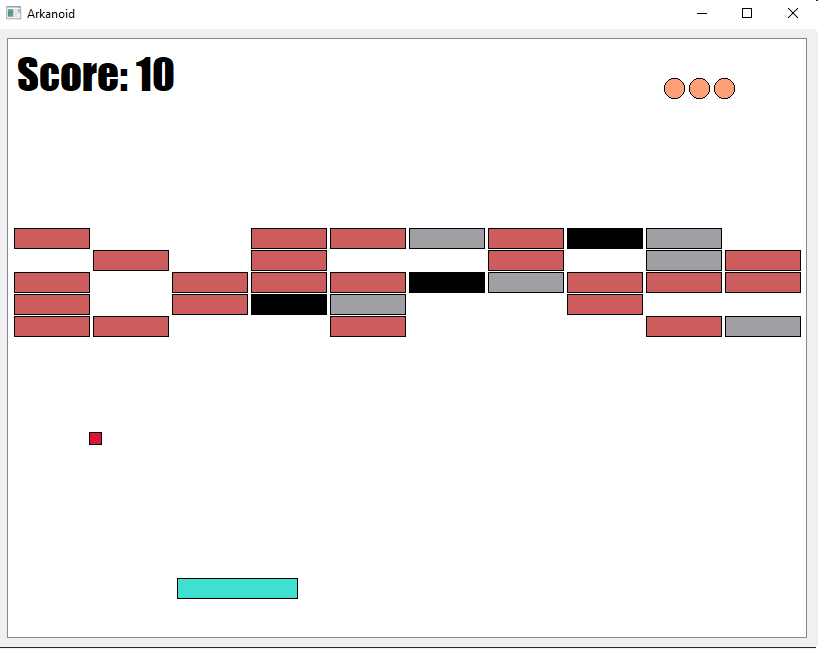
\includegraphics[width=10cm]{image/7.png}
  \caption{окно с игрой (тест подбора бонуса). }
  \label{fig:image}
\end{figure}


Проверка ломания кирпичей мячём.

Убедиться, что кирпич разрушается и исчезает с экрана. Проверить, что счет обновляется в соответствии с типом кирпича (обычный или бонусный).

\begin{figure} [h!]
  \centering
  \graphicspath{ {img/} }
  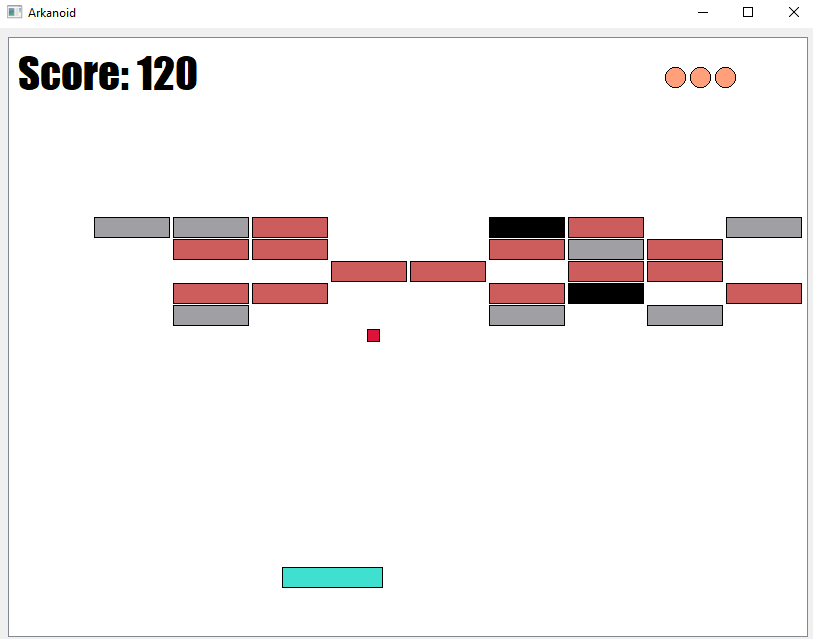
\includegraphics[width=10cm]{image/4.png}
  \caption{окно с игрой (тест кирпичей). }
  \label{fig:image}
\end{figure}
% Подключение третий главы (практическая часть с тестированием):
\chapter{\label{ch:ch03}ГЛАВА 3}

Пример ссылок:
\begin{enumerate}
\item на главу~\ref{ch:ch01};
\item на раздел~\ref{sec:ch01/sec01} главы~\ref{ch:ch01};
\item на раздел~\ref{sec:ch02/sec01} главы~\ref{ch:ch02};
\item на приложение на странице~\pageref{appendix1};
\item на код на странице~\pageref{code:pi-example}.
\end{enumerate}

\section{\label{sec:ch03/sec01}Раздел 1}

\subsection{\label{subsec:ch03/sec01/sub01}Подраздел 1}

\subsection{\label{subsec:ch03/sec01/sub02}Подраздел 2}

\section{\label{sec:ch03/sec02}Раздел 2}

\subsection{\label{subsec:ch03/sec02/sub01}Подраздел 1}

\subsection{\label{subsec:ch03/sec02/sub02}Подраздел 2}




\chapter*{Заключение}
\phantomsection\addcontentsline{toc}{chapter}{ЗАКЛЮЧЕНИЕ}

В процессе разработки курсовой работы была создана игра «Арканоид» на языке программирования Python с использованием библиотеки PySide6. Разработка этой игры стала для меня значимым шагом в изучении новых инструментов и технологий Python, а также в углублении навыков работы с графическим интерфейсом, обработкой событий и анимацией.

Python оправдал свой выбор как отличный инструмент для создания игр благодаря своей простоте и мощным библиотекам, включая PySide6, которая обеспечила удобство и гибкость в создании пользовательского интерфейса игры. Проект «Арканоид» позволил мне углубиться в различные аспекты игровой разработки, такие как управление движением объектов, обнаружение столкновений и управление игровым циклом.

В целом, разработка игры «Арканоид» стала полезным опытом, который не только расширил мои знания в области программирования, но и показал, как важно учитывать пользовательский опыт при создании игр. Полученные знания и навыки станут надёжным фундаментом для моего дальнейшего развития в сфере разработки игр, особенно в контексте быстрого развития игровой индустрии.

\begin{enumerate}
\item Пример ссылки на электронный источник~\cite{wikiRUArkanoid,wikiRUQtDocumentation,wikiRUHabr}.
\item Пример ссылки на книгу одного автора~\cite{book1author}.
\item Пример ссылки на книгу 5-ти и более авторов~\cite{book5author}.
\end{enumerate}

\newpage
\phantomsection\addcontentsline{toc}{chapter}{СПИСОК ИСПОЛЬЗОВАННОЙ ЛИТЕРАТУРЫ}
\printbibliography[title={Список использованной литературы}]

\appendix
\newpage
\chapter*{\raggedleft\label{appendix1}Приложение}
\phantomsection\addcontentsline{toc}{chapter}{ПРИЛОЖЕНИЕ}
%\section*{\centering\label{code:appendix}Текст программы}

\begin{center}
\label{code:appendix}Текст программы
\end{center}

\begin{code}
\captionof*{listing}{\centering\label{code:pi-example}Игра арканоид}
\vspace{-1cm}\inputminted{C}{src/arcanoid.py}
\end{code}

\end{document}

